\section{Machine Learning Model}

Since the data gathered by the sensors are time
series data, we will use Time Series KMeans (TSKM)
algorithm to cluster the data, that is provided in
python by
\href{https://tslearn.readthedocs.io/en/stable/}{\texttt{tslearn}} library.
KMeans algorithm are chosen because it is simple and
easy to implement, and it is also one of the most
popular clustering technique.

To train the model, we used the data gathered by the
sensors for 3 days, as the InfluxDB database stores,
from 2021-05-01 to 2021-05-03. Since the data,
especially from the MQ135 sensor were not too
accurate, we ``smoothened'' the data by using the
\href{https://pandas.pydata.org/docs/reference/api/pandas.DataFrame.rolling.html}{\texttt{rolling}} mean, which saves
the mean of the current rolling window of 120 data. The number
120 is chosen arbitarily to ensure the data is smooth enough,
but not too smooth that it loses its meaning. We also used 2
clusters for the model, as we only need to separate the data
into ``good'' and ``bad'' air quality.

The result of the training can be seen in
\ref{kmeans}. Due to use of clustering algorithm, we could not
determine the exact value of each indicators that is the
discriminant point that separates the ``good'' and ``bad''
air quality, but we can see that the ``good'' air quality is
represented by the lower part, and the ``bad'' air quality is
represented by the upper part.

We then implement the model into the system by passing each
indicators' current average value to the model to determine
the current air quality level of the room. The result of the
model is then used to determine whether the door should be
opened or closed using the following rules:
\begin{enumerate}
      \item If the CO2 level is ``bad'', the door will not be
            opened, since we don't want any toxic particles to
            get in the room.
      \item If the CO2 level is ``good'', we will check the
            next indicators, temperature and humidity. If
            either temperature or humidity is ``bad'', then the
            door will be opened, since we want to get fresh
            air into the room.
      \item If both temperature and humidity are ``good'',
            then the door will not be opened, since the air
            quality is already good.
\end{enumerate}


\begin{figure}
      \centerline{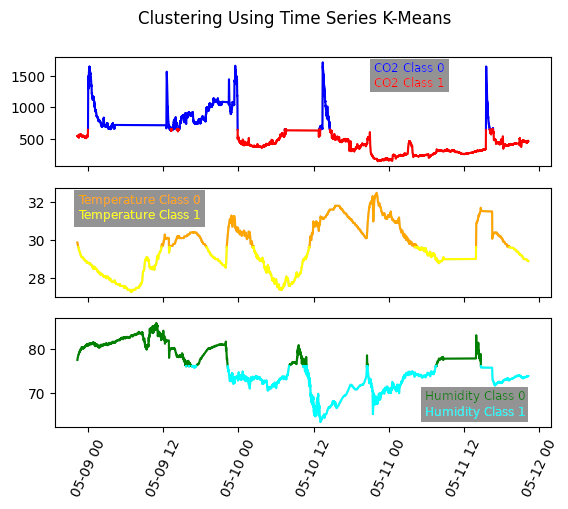
\includegraphics[scale=0.65]{resources/iot-clustering.png}}
      \caption{Time Series KMeans clustering result visualization}
      \label{kmeans}
\end{figure}
